% !TeX root = ../main.tex
\subsection{Hi-C matrices and their patterns} \label{chap: Hi-C matrices}

Hi-C maps are useful tools to detect the interactions occuring inside a genome in analysis. Indeed, they allow to gain insights about the stuctural disposition of chromatin domains, loops and regions.
\cite{lajoieHitchhikerGuideHiC2015}.
The experimental procedure is described in figure \ref{fig: HiC sequencing}. Each position (\textit{i}, \textit{j}) in a Hi-C matrix represents the number of contacts occuring between the coordinates $i^{\text{th}}$ and $j^{\text{th}}$ of the segment. The resolution of an Hi-C map will be dependent on the sequencing process, and have to be decided on the base of the type of information that has to be recovered from the data
\cite{lajoieHitchhikerGuideHiC2015}.

The following list of patterns can be found by inspecting an Hi-C matrix
\cite{distefanoHiCconstrainedPhysicalModels2016,lajoieHitchhikerGuideHiC2015}.

\begin{enumerate}
    \item \textbf{Cis/trans interaction ratio}: There are higher interaction frequencies on average between pairs of \textit{loci} in the same chromosome (\textit{cis}), with respect to those among \textit{loci} which reside on different chromosomes (\textit{trans}). The ratio between \textit{cis/trans} interactions could be indicative of the quality of the obtained Hi-C data.
    The viewed specificity is related to the presence of genomic territories, which govern and establish the disposition of the chromosomes in the nucleus
    \cite{halversonMeltRingsChromosome2014}. The cis-interactions can be easily seen in an Hi-C matrix along the diagonal and are depicted in panel \textit{a} of figure \ref{fig: contact typologies}.
    
    \item \textbf{Distance-dependent interaction frequency}: From the visualization of an Hi-C matrix, it is possible to observe that the largest number of interactions are registered at small distances. On the other hand, only a few contacts can be observed with high spacial separations. Because of this recurring pattern, several studies tried to predict this interesting behavior. Importantly, it was found that in a number of situations it is possible to do that: for example, in yeast the probability of interaction could be described with the following equation
    \cite{lajoieHitchhikerGuideHiC2015}:
    
    $$
        p_{\text{interaction}}(x,y) = Z * \text{dist}(x,y)^{-1,5}
    $$

    Where $\text{dist}(x, y)$ represents the distance between a point \textit{x} and a position \textit{y}.
    
    \item \textbf{Genomic compartments}: Genomic compartments (which can be seen in panel d of figure \ref{fig: contact typologies}) have been found to be correlated with chromatin states, involving DNA accessibility, gene density, replication timing, GC content and histone marks
    \cite{lieberman-aidenComprehensiveMappingLong2009}. 
    The compartments can pertain to two categories, A and B, and are found by performing a principal components analysis with the matrix generated with Pearson Correlation coefficients (a formula for their calculation can be found in chapter \ref{chap: SCC method}). In general A-type compartments are defined as the euchromatic gene-dense regions, while B blocks are defined as gene-poor heterochromatic regions. 
    The positions where they are found differ depending on the type and biological conditions of the analyzed cells
    \cite{lajoieHitchhikerGuideHiC2015}.
    
    \item \textbf{Topological domains}: Also called TADs, they can be visually found in Hi-C matrices as larger squared boxes centered on the diagonal of the maps (panel \textit{b} figure \ref{fig: contact typologies}). They are contiguous portions in which \textit{loci} tend to interact much more with each other than with \textit{loci} outside the region
    \cite{lajoieHitchhikerGuideHiC2015}. 
    It is hypothesized that TADs specify elementary regulatory micro-environments in which promoters interact with local enhancers. Finally, some proteins like cohesins and CTCF tend to interact with the genome at the boundaries of the Topological Domains
    \cite{lajoieHitchhikerGuideHiC2015}.
    
    \item \textbf{Point interactions}: Those are connections occuring between small regions, and involve sequences of a few kb length. Biologically speaking, those points could indicate for example the interactions between enhancers and promoters. When considering a specific point connections, the observed value should be compared to the expected number of interactions for the distance in analysis, and the significance should be computed
    \cite{lajoieHitchhikerGuideHiC2015}.
\end{enumerate}

\begin{figure}[H]
    \centering
    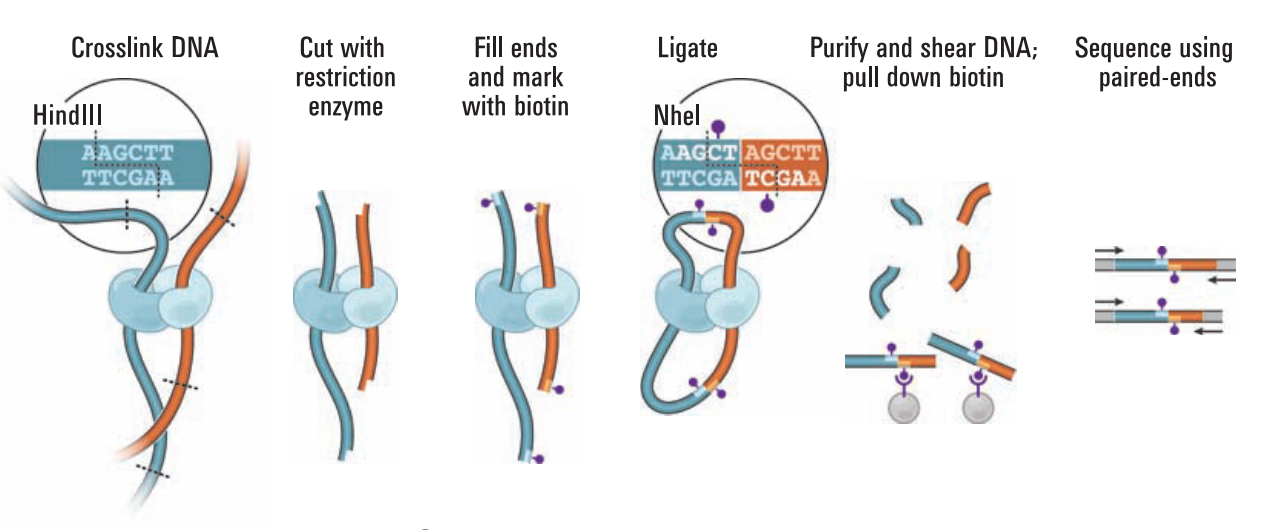
\includegraphics[width=0.7\linewidth]{./images/HiC-seq.png}
    \caption{Image taken from the following \href{https://data.4dnucleome.org/experiment-types/dilution-hi-c/}{link}
    \cite{lieberman-aidenComprehensiveMappingLong2009}, 
    representing the Hi-C sequencing technique in a schematized way.}
    \label{fig: HiC sequencing}
\end{figure}

\begin{figure}[H]
    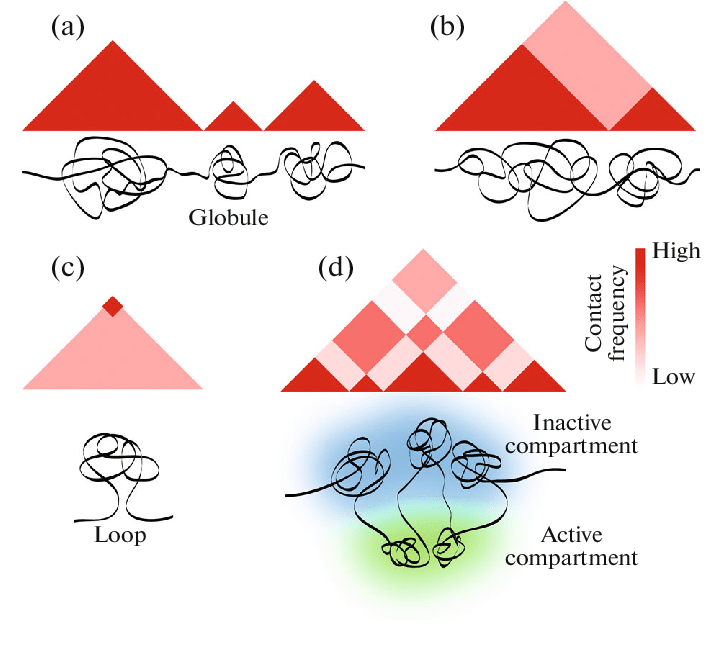
\includegraphics[width=0.55\linewidth]{./images/HiC-contacts.png}
    \caption{The image was taken from the work of Razin and colleagues
    \cite{razin3DGenomics2019}. Figure representing the contact typologies described in this chapter. (a) Isolated triangles on a heat map are commonly interpreted as chromatin globules deriving from cis-interactions. (b) a TAD, represented as a combination of small triangles into larger ones. (c) An intense signal at the apex of a triangle suggests the interaction of TAD boundaries and the formation of a chromatin loop. (d) Representation of some chromatin compartments.}
    \label{fig: contact typologies}
\end{figure}

